\section{Conjugate Gradient Method}\label{sec:cg}
This section is largely based on the extremely instructive book by \citeauthor{iter_method_saad} about iterative methods \cite[Section 6: Krylov Subspace Methods Part I]{iter_method_saad}

The conjugate gradient method is a special instance of a projection method discussed in \cref{sec:projm} where
\begin{equation}
  \mathcal{K}_m(A_0, r_0) = \text{span}\{r_0, Ar_0, A^2r_0, \dots, A^{m-1}r_0\},
  \label{eq:cg_krylov_space}
\end{equation}
or $\mathcal{K}_m$ as a shorthand. The approximate answer is then given by
\begin{equation}
  x_m = x_0 + \sum_{i=0}^{m-1} c_i A^i r_0 = x_0 + q_{m-1}(A)r_0,
  \label{eq:cg_approximate_solution}
\end{equation}
where $q_{m-1}(A)$ is a polynomial of degree $m-1$ in $A$. It is shown later in this section how the coefficients $c_i$ are obtained (\cref{eq:cg_solution_coefficients}).

\subsection{Variants of the CG method} \label{sec:cg_variants}
Variants of the CG method differ in the way A is preconditioned (see section \cref{sec:cg_preconditioning}) d the choices for the constraint subspace $\mathcal{L}_m$. The former type of variations result in the preconditioned CG method PCG and these are described in \cref{sec:cg_preconditioning}. The latter type of variations branch off into two major categories:
\begin{enumerate}[label=\roman*,ref=CG-type \roman*]
  \item\label{cg_type:direct} $\mathcal{L}_m = \mathcal{K}_m$ and $\mathcal{L}_m = A\mathcal{K}_m$;
  \item\label{cg_type:transpose}$\mathcal{L}_m = \mathcal{K}_m(A^T,r_0)$.
\end{enumerate}
Note that \cref{cg_type:direct} correspond to the residual and error projection methods from \cref{sec:projm_projectors}. The former results in Arnoldi's method, which is discussed in \cref{sec:arnoldi}, as well as variants thereof like Full Orthogonalization Method (FOM), Incomplete Orthogonalization Method (IOM) and Direct Incomplete Orthogonalization Method (DIOM). The latter on the other hand results in the Generalized Minimum Residual Method (GMRES).

\subsection{Krylov subspaces}
\begin{definition}
  The grade of a vector $v$ with respect to a matrix $A$ is the lowest degree of the polynomial $q$ such that $q(A)v = 0$.
  \label{def:cg_grade}
\end{definition}
Consequently,
\begin{theorem}
  The Krylov subspace $\mathcal{K}_m$ is of dimension $m$ if and only if the grade $\mu$ of $v$ with respect to $A$ is not less than $m$ \cite[proposition 6.2]{iter_method_saad},
  \begin{equation*}
    \dim(\mathcal{K}_m) = m \iff \mu \geq m,
  \end{equation*}
  such that
  \begin{equation}
    \dim(\mathcal{K}_m) = \min \{m, \textrm{grade}(v)\}.
    \label{eq:cg_krylov_dimension}
  \end{equation}
  \label{th:cg_krylov_dimension}
\end{theorem}

\begin{definition}
  The action of a matrix $A$ can be thought of as a mapping
  \begin{equation*}
    \mathbb{R}^n \rightarrow \mathbb{R}^n: v \mapsto A v
  \end{equation*}
  Thus the domain and codomain of $A$ are $\mathbb{R}^n$. Let $X \subset \mathbb{R}^n$, we can consider the map
  \begin{equation*}
    X \rightarrow \mathbb{R}^n: v \mapsto A v
  \end{equation*}
  instead. The only difference from $A$ is that the domain is $X$. This map is defined as the restriction $A_{\left.\right|_X}$ of $A$ to $X$.
\end{definition}

\begin{definition}
  Let $Q$ be a projector onto the subspace $X$. Then the section of the operator $A$ onto $X$ is defined as $QA_{\left.\right|_X}$.
\end{definition}

\begin{theorem}
  Let $Q_m$ be any projector onto $\mathcal{K}_m$ and let $A_m$ be the section of $A$ to $\mathcal{K}_m$, that is, $A_m=Q_m A_{\left.\right|\mathcal{K}_m}$. Then for any polynomial $q$ of degree not exceeding $m-1$ \cite[proposition 6.3]{iter_method_saad},
  \begin{equation*}
    q(A) v=q\left(A_m\right) v
  \end{equation*}
  and for any polynomial of degree $\leq m$,
  \begin{equation*}
    Q_m q(A) v=q\left(A_m\right) v
  \end{equation*}
\end{theorem}

\begin{figure}[H]
  \centering
  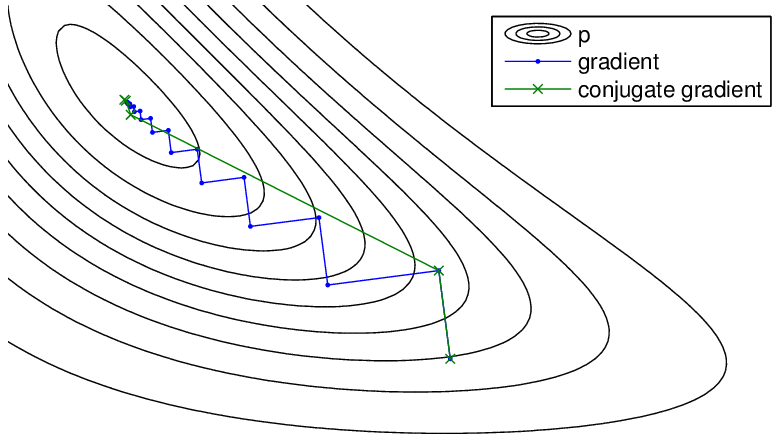
\includegraphics[width=0.5\textwidth]{cg_convergence.png}
  \caption{Conjugate Gradient Method}
  \label{fig:cg}
\end{figure}

\subsection{Arnoldi's method} \label{sec:arnoldi}
The Arnoldi method is a generalization of the Gram-Schmidt orthogonalization process to Krylov subspaces. The Arnoldi method is used to generate an orthonormal basis for the Krylov subspace $\mathcal{K}_m(A, r_0)$.
\begin{algorithm}[H]
  \caption{Arnoldi's method \cite[Algorithm 6.1]{iter_method_saad}}
  \begin{algorithmic}
    \State Choose a vector $v_1$ with $||v_1|| = 1$
    \For{$j = 1, 2, \dots, m$}
    \State $w_j \leftarrow Av_j$
    \For{$i = 1, 2, \dots, j$}
    \State $h_{ij} \leftarrow (w, v_i)$
    \State $w_j \leftarrow w_j - h_{ij}v_i$
    \EndFor
    \State $h_{j+1,j} \leftarrow ||w_j||$
    \State $v_{j+1} \leftarrow w_j / h_{j+1,j}$
    \EndFor
  \end{algorithmic}
  \label{alg:arnoldi}
\end{algorithm}
The Arnoldi method generates an orthonormal basis $V_m = [v_1, v_2, \dots, v_m]$ for the Krylov subspace $\mathcal{K}_m(A, r_0)$ and an upper Hessenberg matrix $\bar{H}_m$ such that
\begin{subequations}\label{eq:arnoldi_decomposition}
  \begin{align}
    AV_m      & = V_m H_m + h_{m+1,m}v_{m+1}e_m^T \label{eqn:arnoldi_decomposition0}, \\
              & = V_{m+1}\bar{H}_m, \label{eqn:arnoldi_decomposition1},               \\
    V^T_mAV_m & = H_m, \label{eqn:arnoldi_decomposition2}
  \end{align}
\end{subequations}
where $e_m$ is the $m$th unit vector and $H_m$ is obtained from $\bar{H}_m$ by removing the last row \cite[Proposition 6.5]{iter_method_saad}.

Note that the Arnoldi method stops at $j$, if and only if the minimal polynomial of $A$ with respect to $v_1$ is of degree $j$ \cite[proposition 6.6]{iter_method_saad}.

\subsection{Arnoldi's method for linear systems}\label{sec:arnoldi_linear_systems}
The Arnoldi method can be used to solve linear systems of the form $Ax = b$. If $v_1 = r_0/||r_0||_2$ and $\beta = ||r_0||_2$, then by \cref{eqn:arnoldi_decomposition2} we have
\[
  V^T_mAV_m = H_m \text{ and } V^T_mr_0 = V^T_m\beta v_1 = \beta e_1 \implies \begin{array}{c}
    H_m y = \beta e_1, \\
    x_m = x_0 + V_m y.
  \end{array} .
\]
This results in the following algorithm
\begin{algorithm}[H]
  \caption{Arnoldi's method for linear systems (FOM) \cite[Algorithm 6.4]{iter_method_saad}}
  \label{alg:arnoldi_linear_systems}
  \begin{algorithmic}
    \State Compute $r_0 = b - Ax_0$, $\beta = ||r_0||_2$ and $v_1 = r_0 / \beta$
    \State Define $H_m = \{0\}$
    \State Define $V_1 = \{v_1\}$
    \For{$j = 1, 2, \dots, m$}
    \State $w_j = Av_j$
    \For{$i = 1, 2, \dots, j$}
    \State $h_{ij} = (w_j, v_i)$ and store $h_{ij}$ in $H_m$
    \State $w_j = w_j - h_{ij}v_i$
    \EndFor
    \State $h_{j+1,j} = ||w_j||_2$
    \If{$h_{j+1,j} = 0$}
    \State $m = j$
    \State break
    \EndIf
    \State $v_{j+1} = w_j / h_{j+1,j}$ and store $v_{j+1}$ into $V_{j+1}$
    \EndFor
    \State Solve $H_m y_m = \beta e_1$ for $y_m$
    \State $x_m = x_0 + V_m y_m$
  \end{algorithmic}
\end{algorithm}

Note that a stopping criterion can be derived from the residual vector $r_m = b - Ax_m$. Theorem \ref{th:arnoldi_residual} gives a way of calculating the size of the residual vector.
\begin{theorem}
  The residual vector $r_m = b - Ax_m$ satisfies
  \begin{subequations}
    \begin{align}
      r_m                                          & = b - Ax_m                                                  \\
                                                   & = r_0 - AV_m y_m                                            \\
      \cref{eqn:arnoldi_decomposition0}\rightarrow & = \beta v_1 - V_m H_m y_m - h_{m+1,m} e_m^T y_m v_{m+1}     \\
                                                   & = - h_{m+1,m} e_m^T y_m v_{m+1}.\label{eq:arnoldi_residual}
    \end{align}
  \end{subequations}
  Therefore, the residual vector is orthogonal to the Krylov subspace $\mathcal{K}_m(A, r_0)$ and its size is given by
  \begin{equation}
    ||r_m||_2 = h_{m+1,m}|e^T_m y_m|,
    \label{eq:arnoldi_residual_size}
  \end{equation}
  where $h_{m+1,m}\geq 0$ \cite[Proposition 6.7]{iter_method_saad}.
  \label{th:arnoldi_residual}
\end{theorem}

\subsection{Lanczos' Algorithm}
In the special case where $A$ is symmetric, the Arnoldi method can be simplified to the Lanczos algorithm. The Lanczos algorithm is a special case of the Arnoldi method where the matrix $T_m = V^T_mAV^T_m$ is tridiagonal given by
\begin{equation}
  T_m =
  \begin{pmatrix}
    \delta_1 & \eta_2   & 0        & \dots  & 0        \\
    \eta_2   & \delta_3 & \eta_3   & \dots  & 0        \\
    0        & \eta_3   & \delta_4 & \dots  & 0        \\
    \vdots   & \vdots   & \vdots   & \ddots & \eta_m   \\
    0        & 0        & 0        & \eta_m & \delta_m
  \end{pmatrix}
  \label{eq:lanczos_tridiagonal}
\end{equation}
This leads to the following algorithm
\begin{algorithm}[H]
  \caption{Lanczos \cite[algorithm 6.15]{iter_method_saad}}
  \begin{algorithmic}
    \State Choose a vector $v_1$ with $||v_1|| = 1$
    \State $\eta_1 = 0$
    \State $v_0 = 0$
    \For{$j = 1, 2, \dots, m$}
    \State $w_j = Av_j - \eta_j v_{j-1}$
    \State $\delta_j = (w_j, v_j)$
    \State $w_j = w_j - \delta_j v_j$
    \State $\eta_{j+1} = ||w_j||$
    \If{$\eta_{j+1} = 0$}
    \State Break
    \EndIf
    \State $v_{j+1} = w_j / \eta_{j+1}$
    \EndFor
  \end{algorithmic}
\end{algorithm}
Similarly, we can apply the Lanczos algorithm to linear systems resulting in \cref{alg:lanczos_linear_systems}.
\begin{algorithm}
  \caption{Lanczos algorithm for linear systems \cite[Algorithm 6.16]{iter_method_saad}}
  \begin{algorithmic}
    \State Compute $r_0 = b - Ax_0$, $\beta = ||r_0||_2$, $v_0 = 0$ and $v_1 = r_0 / \beta$
    \State $V_{1} = \{v_1\}$
    \For{$j = 1, 2, \dots, m$}
    \State $w_j = Av_j - \eta_j v_{j-1}$
    \State $\delta_j = (w_j, v_j)$
    \State $w_j = w_j - \delta_j v_j$
    \State $\eta_{j+1} = ||w_j||_2$
    \If{$\eta_{j+1} = 0$}
    \State $m = j$
    \State Break
    \EndIf
    \State $v_{j+1} = w_j / \eta_{j+1}$ and store $v_{j+1}$ into $V_{j+1}$
    \EndFor
    \State Solve the tridiagonal system $T_m y_m = \beta e_1$ for $y_m$
    \State $x_m = x_0 + V_m y_m$
  \end{algorithmic}
  \label{alg:lanczos_linear_systems}
\end{algorithm}

\subsection{D-Lanczos} The direct version of the Lanczos algorithm or `D-Lanczos' is obtained by performing a LU-factorisation $T_m$
\begin{equation}
  T_m = L_m U_m =
  \begin{pmatrix}
    1              & 0              & 0      & \dots          & 0      \\
    \tilde{\eta}_2 & 1              & 0      & \dots          & 0      \\
    0              & \tilde{\eta}_3 & 1      & \dots          & 0      \\
    \vdots         & \vdots         & \vdots & \ddots         & \vdots \\
    0              & 0              & \dots  & \tilde{\eta}_m & 1
  \end{pmatrix}
  \times
  \begin{pmatrix}
    \tilde{\delta}_1 & \eta_2           & 0                & \dots  & 0                \\
    0                & \tilde{\delta}_2 & \eta_3           & \dots  & 0                \\
    0                & 0                & \tilde{\delta}_3 & \dots  & 0                \\
    \vdots           & \vdots           & \vdots           & \ddots & \eta_m           \\
    0                & 0                & 0                & \dots  & \tilde{\delta}_m
  \end{pmatrix}
  \label{eq:lanczos_lu}
\end{equation}
Then, the approximate solution is given by
\begin{align*}
  x_m & = x_0 + V_m y_m                           \\
      & = x_0 + V_m U_m^{-1} L_m^{-1} \beta e_1   \\
      & = x_0 + V_m U_m^{-1} (L_m^{-1} \beta e_1) \\
      & = x_0 + P_m z_m,
\end{align*}
where $P_m = V_m U_m^{-1}$ and $z_m = L_m^{-1} \beta e_1$. Considering the definition of $U_m$ in \cref{eq:lanczos_lu}, we have that the $m^{\text{th}}$ column of $P_m$ is given by
\begin{equation}
  p_m = \frac{1}{\tilde{\delta}_m}\left[v_m - \eta_m p_{m-1}\right].
  \label{eq:lanczos_p}
\end{equation}
Furthermore, from the LU factorization of $T_m$ we have that
\begin{align*}
  \tilde{\eta}_m   & = \frac{\eta_m}{\tilde{\delta}_{m-1}},       \\
  \tilde{\delta}_m & = \delta_m - \tilde{\eta}_m \eta_m, \ m > 1.
\end{align*}
Now the solution can be incrementally updated by realizing that
\[
  z_m =
  \begin{pmatrix}
    z_{m-1} \\
    \zeta_m
  \end{pmatrix} =
  \begin{pmatrix}
    z_{m-2}     \\
    \zeta_{m-1} \\
    \zeta_m
  \end{pmatrix},
\]
and
\[
  L_m =
  \begin{pmatrix}
    L_{m-1}            & \multicolumn{2}{c}{\mathbf{0}_{m-1}}     \\
    \mathbf{0}_{m-2}^T & \tilde{\eta}_m                       & 1
  \end{pmatrix}.
\]
Then,
\[
  L_m z_m =
  \begin{pmatrix}
    L_{m-1} z_{m-1} \\
    \tilde{\eta}_m \zeta_{m-1} + \zeta_m
  \end{pmatrix} =
  \begin{pmatrix}
    \beta e_1 \\
    0
  \end{pmatrix},
\]
where the last equality follows from definition of $z_m$. Consequently, we have that
\[
  \zeta_m = -\tilde{\eta}_m \zeta_{m-1}.
\]
Finally, we obtain
\begin{align*}
  x_m & = x_0 + P_m z_m                                   \\
      & = x_0 + \left[P_{m-1} \ p_m\right] \begin{pmatrix}
                                             z_{m-1} \\
                                             \zeta_m
                                           \end{pmatrix} \\
      & = x_0 + P_{m-1}z_{m-1} + p_m \zeta_m              \\
      & = x_{m-1} + p_m \zeta_m.
\end{align*}
Putting it all together, we obtain \cref{alg:dlanczos}.
\begin{algorithm}[H]
  \caption{D-Lanczos \cite[Algorithm 6.17]{iter_method_saad}}
  \begin{algorithmic}
    \State $r_0 = b - Ax_0$, $\beta = ||r_0||_2$, $v_1 = r_0 / \beta$
    \State $\tilde{\eta}_1 = \beta_1 = 0$, $p_0 = 0$
    \For{$m = 1, 2, \dots, m$ until convergence}
    \State $w = Av_m - \beta_m v_{m-1}$
    \State $\delta_m = (w, v_m)$
    \If{$m > 1$}
    \State $\tilde{\eta}_m = \frac{\beta_m}{\tilde{\delta}_{m-1}}$
    \State $\zeta_m = -\tilde{\eta}_m \zeta_{m-1}$
    \EndIf
    \State $\tilde{\delta}_m = \delta_m - \tilde{\eta}_m \beta_m$
    \State $p_m = \frac{1}{\tilde{\delta}_m}\left[v_m - \beta_m p_{m-1}\right]$
    \State $x_m = x_{m-1} + p_m \zeta_m$
    \If{convergence criterion is met (using \cref{eq:arnoldi_residual_size} for example)}
    \State break
    \EndIf
    \State $w = w - \delta_m v_m$
    \State $\beta_{m+1} = ||w||_2$
    \State $v_{m+1} = w / \beta_{m+1}$
    \EndFor
  \end{algorithmic}
  \label{alg:dlanczos}
\end{algorithm}
Note that the residual vectors produced by \cref{alg:dlanczos} are orthogonal to each other due to \cref{th:arnoldi_residual}. Additionally,
\begin{align*}
  P^T_m A P_m & = U_m^{-T} V_m^T A V_m U_m^{-1} \\
              & = U_m^{-T} T_m U_m^{-1}         \\
              & = U_m^{-T} L_m,
\end{align*}
where $U_m^{-T}$ and $L_m$ are both lower diagonal matrices. Their product must be symmetric, since $P^T_m A P_m$ is (symmetry of $A$). Therefore, $U_m^{-T} L_m$ must be a diagonal matrix. Consequently, the vectors $p_m$ are $A$-orthogonal to each other.

\subsection{Derivation of CG}
From observations made in the in \cref{alg:dlanczos}, we can derive the conjugate gradient method. We start by constraining subsequent residuals $r_j$ to be orthogonal and search directions $p_j$ to be $A$-orthogonal to each other. To that end, let
\begin{equation}
  x_{j+1} = x_j + \alpha_j p_j,
  \label{eq:cg_solution_update}
\end{equation}
and, thereby,
\begin{equation}
  r_{j+1} = r_j - \alpha_j A p_j.
  \label{eq:cg_residual_update}
\end{equation}
If the residuals are to be orthogonal, then
\[
  (r_{j+1}, r_j) = 0 \implies (r_j - \alpha_j A p_j, r_j) = 0 \implies \alpha_j = \frac{(r_j, r_j)}{(A p_j, r_j)}.
\]
Now, using \cref{eq:lanczos_p,eq:arnoldi_residual}, we can write the next search direction as a linear combination of the previous search direction and the next residual
\begin{equation}
  p_{j+1} = r_{j+1} + \beta_j p_j.
  \label{eq:cg_search_direction_update}
\end{equation}
Substituting \cref{eq:cg_search_direction_update}, we obtain
\[
  (Ap_{j+1}, r_j) = (Ap_j, p_j -\beta_{j-1}p_{j_1}) = (Ap_j, p_j),
\]
since $p_j$ is $A$-orthogonal to $p_{j-1}$. This allows us to write
\begin{equation}
  \alpha_j = \frac{(r_j, r_j)}{(A p_j, p_j)}.
  \label{eq:cg_alpha}
\end{equation}
Additionally, taking the inner product with $A p_j$ on both sides of \cref{eq:cg_search_direction_update} gives
\[
  \beta_j = \frac{(r_{j+1}, A p_j)}{(p_j, A p_j)}.
\]
Now, rewriting \cref{eq:cg_residual_update} gives
\[
  Ap_j = \frac{1}{\alpha_j} (r_j - r_{j+1}),
\]
which we substitute into the equation for $\beta_j$ to obtain
\begin{equation}
  \beta_j = \frac{1}{\alpha_j}\frac{(r_{j+1}, (r_{j+1}-r_j))}{(Ap_j, r_j)} = \frac{(r_{j+1},r_{j+1})}{((r_j - r_{j-1}), r_j)} = \frac{(r_{j+1},r_{j+1})}{(r_j, r_j)}.
  \label{eq:cg_beta}
\end{equation}
Finally, we can write the conjugate gradient method as \cref{alg:cg}.
\begin{algorithm}[H]
  \caption{Conjugate Gradient Method \cite[Algorithm 6.18]{iter_method_saad}}
  \begin{algorithmic}
    \State $r_0 = b - Ax_0$, $p_0 = r_0$, $\beta_0 = 0$
    \For{$j = 0, 1, 2, \dots, m$}
    \State $\alpha_j = (r_j, r_j) / (A p_j, p_j)$
    \State $x_{j+1} = x_j + \alpha_j p_j$
    \State $r_{j+1} = r_j - \alpha_j A p_j$
    \State $\beta_j = (r_{j+1}, r_{j+1}) / (r_j, r_j)$
    \State $p_{j+1} = r_{j+1} + \beta_j p_j$
    \EndFor
  \end{algorithmic}
  \label{alg:cg}
\end{algorithm}

\paragraph{Hessenberg matrix coefficients} The coefficients of the Hessenberg matrix $T_m$ can be calculated as follows
\begin{equation}
  \delta_{j+1} =
  \begin{cases}
    \frac{1}{\alpha_j} + \frac{\beta_{j-1}}{\alpha_{j-1}} & j > 0, \\
    \frac{1}{\alpha_0}                                    & j = 0,
  \end{cases}
  \label{eq:cg_hessenberg_delta}
\end{equation}
and
\begin{equation}
  \eta_{j+1} = \frac{\sqrt{\beta_{j-1}}}{\alpha_{j-1}}.
  \label{eq:cg_hessenberg_eta}
\end{equation}
here we have used the definition of $T_m = V_m^T A V_m$ and the fact that the residuals are just multiples of the Lanczos vectors $r_j = \text{scalar} \times v_j$ by \cref{eq:arnoldi_residual} \cite[Equation 6.103]{iter_method_saad}.

\subsection{Convergence of CG}
\subsubsection{Convergence rate}\label{sec:cg_convergence_rate}
It can be shown \cite[lemma 6.28 and theorem 6.29]{iter_method_saad} that the error of the $m^{\text{th}}$ iterate of the CG algorithm $\epsilon_m = x^* - x_m$ minimizes the $A$-norm of the error in the affine Krylov subspace $\mathcal{K}_m(A, r_0)$, that is
\[
  ||(I - Aq_m(A))\epsilon_0||_A = \min_{q \in \mathcal{P}_{m-1}} ||(I - Aq(A))\epsilon_0||_A = \min_{r \in \mathcal{P}_{m-1}, r(0) = 1} ||r(A)\epsilon_0||_A,
\]
where the equality follows, since there exists an isomorphic mapping between the affine Krylov subspace and the polynomial space $\mathcal{P}_{m-1}$ of degree $m-1$ and the polynomial $tq(t)$ equals $0$ at $t=0$. The right-hand side can be further bounded by letting $\lambda_i, \xi_i$ be the eigenvalues of $A$ and the components of $\epsilon_0$ in the eigenvector basis of $A$, respectively. Then
\[
  ||r(A)\epsilon_0||_A = \sqrt{\sum_{i=1}^n |r(\lambda_i)|^2 |\xi_i|^2} \leq \max_{\lambda \in \sigma(A)} |r(\lambda)| ||\epsilon_0||_A,
\]
where $\sigma(A)$ is the spectrum of $A$. This gives
\begin{align*}
  ||e_m||                                                                                                                            & \leq \min_{r \in \mathcal{P}_{m-1}, r(0) = 1} \max_{\lambda \in \sigma(A)} |r(\lambda)| ||\epsilon_0||_A \\
  \text{Chebyshev polynomial } C_m \text{, } \eta=\frac{\lambda_{\text{min}}}{\lambda_{\text{max}}-\lambda_{\text{min}}} \rightarrow & \frac{||\epsilon_0||_A}{C_m(1+2\eta)}                                                                    \\
                                                                                                                                     & \leq \frac{2||\epsilon_0||_A}{\left(1 + 2\eta + 2\sqrt{\eta(\eta+1)}\right)^m}                           \\
                                                                                                                                     & = \frac{2||\epsilon_0||_A}{\left(\sqrt{\eta} + \sqrt{\eta + 1}\right)^{2m}}                              \\
                                                                                                                                     & = 2 \left(\frac{\sqrt{\kappa}-1}{\sqrt{\kappa} + 1}\right)^m ||\epsilon_0||_A,
\end{align*}
where $\kappa = \lambda_{\text{max}}/\lambda_{\text{min}}$ is the condition number of (symmetric matrix) $A$. To sum up
\begin{theorem}
  The error of the $m^{\text{th}}$ iterate of the CG algorithm is bounded by
  \begin{equation}
    ||e_m|| \leq 2 \left(\frac{\sqrt{\kappa}-1}{\sqrt{\kappa} + 1}\right)^m ||\epsilon_0||_A,
    \label{eq:cg_convergence_rate}
  \end{equation}
  where $\kappa = \lambda_{\text{max}}/\lambda_{\text{min}}$ is the condition number of (symmetric matrix) $A$.
  \label{th:cg_convergence_rate}
\end{theorem}
During the derivation of \cref{th:cg_convergence_rate}, we obtain the general expression for the error of the $m^{\text{th}}$ iterate of the CG algorithm
\[
  || e_m|| \leq \min_{r \in \mathcal{P}_{m}, r(0) = 1} \max_{\lambda \in \sigma(A)} |r(\lambda)| ||\epsilon_0||_A \\
\]
Now define,
\[
  r_{\textrm{test}}(t) = \prod_{i=1}^m \frac{\lambda_i - t}{\lambda_i}.
\]
Note that $r_{\textrm{test}}\in\mathcal{P}_m$, since it has degree $m$. Also, $r_{\textrm{test}}(0) = 1$ and $r_{\textrm{test}}(\lambda_i) = 0$ for $i = 1, 2, \dots, m$. Hence, $r_{\textrm{test}}$ is a polynomial that satisfies the constraints of the minimization problem. We obtain for $m = N$ that
\[
  ||e_N||_A = ||\epsilon_0||_A \max_{\lambda \in \sigma(A)} |r_{\textrm{test}}(\lambda)| = 0,
\]
which implies that CG converges in $N$ iterations in exact arithmetic. Furthermore, if there are only $k$ distinct eigenvalues, then the CG iteration terminates in at most $k$ iterations.

\subsubsection{Condition number estimation} \label{sec:cg_condition_number_estimate}
During CG iterations it is possible to get an estimate of the condition number of the matrix $A$ by using the tridiagonal Hessenberg matrix $T_m$ and the recurrence relation for determinant of tridiagonal matrices. Suppose the characteristic polynomial of $T_j$ is given by $p_{T_j}(\lambda)$, then
\begin{align*}
  p_{T_0}(\lambda) & = 1,                                                                   \\
  p_{T_1}(\lambda) & = \lambda - \delta_1,                                                  \\
  p_{T_2}(\lambda) & = (\lambda - \delta_2)p_{T_1}(\lambda) - \eta_2^2,                     \\
  p_{T_3}(\lambda) & = (\lambda - \delta_3)p_{T_2}(\lambda) - \eta_3^2(\lambda - \delta_1), \\
                   & \vdots                                                                 \\
\end{align*}
Hence, the characteristic polynomial of $T_j$ can be written as
\begin{align}
  p_{T_j}(\lambda) & = (\lambda - \delta_j)p_{T_{j-1}}(\lambda) - \eta_j^2p_{T_{j-2}}
  \label{eq:cg_hessenberg_char_poly}.
\end{align}
Now the condition number of $A$ is defined as
\[
  \kappa(A) = ||A||_2 ||A^{-1}||_2 = \max_{x\in\mathbb{R}^n, x\neq0} \frac{||Ax||_2}{||x||_2} \max_{x\in\mathbb{R}^n, x\neq0} \frac{||A^{-1}x||_2}{||x||_2}.
\]
Similarly, the condition number of $T_j$ is defined as
\[
  \kappa(T_j) = ||T_j||_2 ||T_j^{-1}||_2 = \max_{x\in\mathbb{R}^j, x\neq0} \frac{||T_jx||_2}{||x||_2} \max_{x\in\mathbb{R}^j, x\neq0} \frac{||T_j^{-1}x||_2}{||x||_2}.
\]
Note that
\begin{align*}
  \max_{x\in\mathbb{R}^j, x\neq0} \frac{||T_jx||_2}{||x||_2} & = \max_{x\in\mathbb{R}^n, x\neq0} \frac{||V_j^T A V_j x||_2}{||x||_2}                        \\
  \text{orthogonality of } V_j \rightarrow                   & = \max_{x\in\mathbb{R}^n, x\neq0} \frac{||V_j(V_j^T A V_j x)||_2}{||V_j x||_2}               \\
                                                             & = \max_{x\in\mathbb{R}^j, x\neq0} \frac{||A V_j x||_2}{||V_j x||_2}                          \\
                                                             & = \max_{\tilde{x}\in\mathcal{K}_j, \tilde{x}\neq0} \frac{||A \tilde{x}||_2}{||\tilde{x}||_2} \\
                                                             & \approx ||A||_2,
\end{align*}
and similarly for the inverse. Presumably, the estimate will get better as $j$ increases and the Krylov subspace $\mathcal{K}_j$ gets closer to the eigenspace of $A$. \todo{Find proof of this}.

Now, combining this with the recurrence relation for the characteristic polynomial of $T_j$ in \cref{eq:cg_hessenberg_char_poly}, we have a way of estimating the condition number of $A$. In particular, at any iteration $j$ of the CG algorithm, let $\tilde{\lambda}_{\text{max}}$ and $\tilde{\lambda}_{\text{min}}$ be the maximum and minimum zeroes of $p_{T_j}$. Then, the condition number of $A$ is approximately given by
\begin{equation}
  \kappa(A) \approx \frac{\tilde{\lambda}_{\text{max}}}{\tilde{\lambda}_{\text{min}}}.
  \label{eq:cg_condition_number_estimate}
\end{equation}

\subsubsection{Influence of eigenvalue distribution on convergence}\label{sec:cg_eigenvalue_distribution}
In the derivation of the convergence rate of the CG algorithm in \ref{th:cg_convergence_rate}, we used the Chebyshev polynomial to bound the error. However, we can find an expression of the error provided the eigendecomposition of $A$ is available. Suppose $A = VDV^T$, then $r(A) = I - Aq(A) = V(I - Dq(D))V^T = Vr(D)V^T$. Also note that $e_0 = x^* - x_0 = A^{-1}b - x_0 = A^{-1}r_0$. As seen in \cref{sec:cg_convergence_rate}, the error of the $m^{\text{th}}$ iterate of the CG algorithm is given by
\begin{equation*}
  ||e_m||_A^2 = ||r_m(A)\epsilon_0||_A^2,
\end{equation*}
and
\begin{align*}
  ||r_m(A)\epsilon_0||_A^2 & = \epsilon_0^T r_m(A)^T A r_m(A) \epsilon_0                 \\
                           & = \epsilon_0^T V r_m(D) V^T V D V^T V r_m(D) V^T \epsilon_0 \\
                           & = (V^T\epsilon_0)^T r_m(D) D r_m(D) V^T \epsilon_0.
\end{align*}
We also have
\begin{align*}
  V^T\epsilon_0 & = V^T A^{-1} r_0       \\
                & = V^T V D^{-1} V^T r_0 \\
                & = D^{-1} \rho_0,
\end{align*}
where $\rho_0 = V^T r_0$ is the initial residual in the eigenvector basis of $A$. Therefore,
\begin{align*}
  ||r_m(A)\epsilon_0||_A^2 & = \rho_0^T D^{-1} r_m(D) D r_m(D) D^{-1} \rho_0                 \\
                           & = \rho_0^T r_m(D) D^{-1} r_m(D)  \rho_0                         \\
                           & = \sum_{i=1}^n \frac{r_m(\lambda_i)^2}{\lambda_i} \rho_{0,i}^2,
\end{align*}
which gives
\begin{equation}
  ||e_m||_A^2 = \sum_{i=1}^n \frac{r_m(\lambda_i)^2}{\lambda_i} \rho_{0,i}^2.
  \label{eq:cg_error_eigenvalue}
\end{equation}

To obtain the residual polynomial $r_m$, we can use the recurrence relation between the Lanczos vectors and expressions for the Hessenberg matrix coefficients in \cref{eq:cg_hessenberg_delta,eq:cg_hessenberg_eta}. In particular,
\begin{align*}
  \frac{1}{\eta_{j+1}} v_j & = A v_j - \delta_j v_j - \eta_j v_{j-1} \\
                           & = p_{j+1}(A) v_1,
\end{align*}
where we define $p_{-1}(A) = 0, p_0(A) = I$. This gives
\begin{align*}
  \eta_{j+1}p_{j+1}(A)v_1 & = A v_j - \delta_j v_j - \eta_j v_{j-1},                            \\
                          & = \left( A p_j(A) - \delta_j p_j(A) - \eta_j p_{j-1}(A) \right)v_1, \\
\end{align*}
and therefore
\begin{equation}
  p_{j+1}(A) = \frac{1}{\eta_{j+1}}\left( (A - \delta_j )p_j(A) - \eta_j p_{j}(A) \right).
  \label{eq:cg_lanczos_polynomial}
\end{equation}
Furthermore, we have the following relation between the residual polynomial and the Lanczos polynomial \cite[Section 3.2]{Meurant_Strakoš_2006}
\begin{equation}
  r_{j}(A) = (I-Aq_{j-1}(A))r_0 = \frac{p_{j}(A)}{p_{j}(0)}r_0.
  \label{eq:cg_residual_polynomial}
\end{equation}
This gives a way of calculating the residual polynomial $r_m$ and thereby the error of the $m^{\text{th}}$ iterate of the CG algorithm.

Additionally, the coefficients $c_i$ of the solution polynomial $q_m$ in \cref{eq:cg_approximate_solution} can be calculated. First we introduce a function that extracts the coefficients of a polynomial $p$
\begin{definition}
  Let $p(t) = \sum_{i=0}^n c_i t^i$ be a polynomial of degree $n$. Then, the function $\text{coeff}(p;i)$ extracts the $i^{\text{th}}$ coefficient of $p$ such that $\text{coeff}(p;i) = c_i$.
\end{definition}
Now using \cref{eq:cg_residual_polynomial}, we can write the solution polynomial as
\begin{align*}
                              & Aq_{m-1}(A) = I - r_m(A)                                                  \\
  r_m(\mathbf{0}) = I\implies & A\sum_{i=1}^{m-1} c_{i-1} A^i = -\sum_{i=1}^{m} \text{coeff}(r_m; i) A^i,
\end{align*}
which implies
\begin{equation}
  c_i = -\text{coeff}(r_m; i+1), \quad i = 0, 1, \dots, m-1.
  \label{eq:cg_solution_coefficients}
\end{equation}
\begin{figure}[H]
  \centering
  \includegraphics[width=\textwidth]{cg_convergence_behaviour.pdf}
  \caption{Residual polynomials resulting from successive CG iterations}
  \label{fig:cg_convergence_behaviour}
\end{figure}

The behavior of the residual polynomials is crucial for understanding the convergence properties of the CG method. In particular, the distribution of the eigenvalues of $A$ significantly affects the convergence rate, as illustrated in \cref{fig:cg_effect_of_eigenvalue_distribution}.
\begin{figure}[H]
  \centering
  \includegraphics[width=\textwidth]{effect_of_eigenvalue_distribution.pdf}
  \caption{Plots of the last three CG residual polynomials for different eigenvalue distributions. $n_c$ indicates  the number of clusters and $\sigma$ is the width of the cluster. The size of the system $n$ and the condition number $\kappa(A)$ are kept constant.}
  \label{fig:cg_effect_of_eigenvalue_distribution}
\end{figure}
Hence, the number of iterations required for convergence depends on the specific clustering of the eigenvalues, as pointed out for example in \citeauthor[Section 2.3]{nonlinear_cg_Kelley_1995}.

From the behavior exhibited in figure \cref{fig:cg_effect_of_eigenvalue_distribution} as well as from \cref{th:cg_krylov_dimension} we can reason what the best and worst possible spectra for CG convergence are. That is, the best possible spectrum is one where eigenvalues are tightly clustered around distinct values, while the worst possible spectrum is one where the eigenvalues are evenly distributed across the whole range of the spectrum. This is illustrated in \cref{fig:cg_best_worst_spectra}.
\begin{figure}[H]
  \centering
  \includegraphics[width=\textwidth]{cg_convergence_extreme_spectra.pdf}
  \caption{Best and worst possible spectra for CG convergence}
  \label{fig:cg_best_worst_spectra}
\end{figure}

\subsection{Preconditioning} \label{sec:cg_preconditioning}
Suppose $M$ is some SPD preconditioner, then variants of CG can be derived by applying $M$ to the system of equations. The three main approaches are
\begin{enumerate}[label=\roman*,ref=preconditioner-type \roman*]
  \item\label{pcg_type:left} left
  \begin{align*}
    M^{-1}Ax & = M^{-1}b
  \end{align*}
  \item\label{pcg_type:right} right
  \begin{align*}
    AM^{-1}u & = M^{-1}b  \\
    x        & = M^{-1}u;
  \end{align*}
  \item\label{pcg_type:symmetric} symmetric or split
  \begin{align*}
    M              & = LL^T     \\
    x              & = L^{-T}u  \\
    L^{-1}AL^{-T}u & = L^{-1}b.
  \end{align*}
\end{enumerate}
Furthermore, all these variants are mathematically equivalent in some sense. Indeed, for the cases \cref{pcg_type:left} and \cref{pcg_type:right}, we can rewrite the CG algorithm using the $M-$ or $M^{-1}-$inner products, respectively. In either case the iterates are the same. For instance for the left preconditioned CG, we define $z_j = M^{-1}r_j$. Note that $M^{-1}A$ is self-adjoint with respect to the $M-$inner product, that is
\[
  (M^{-1}Ax, y)_M = (Ax, y) = (x, Ay) = (x, M^{-1}Ay)_M.
\]
We use this to get a new expression for $\alpha_j$. To that end, we write
\begin{align*}
  0 & = (r_{j+1}, r_j)_M                                        \\
    & = (z_{j+1}, r_j)                                          \\
    & = (z_j - \alpha_j M^{-1}Ap_j, M^{-1}r_j)_M                \\
    & = (z_j, M^{-1}r_j)_M - \alpha_j (M^{-1}Ap_j, M^{-1}r_j)_M \\
    & = (z_j, z_j)_M - \alpha_j (M^{-1}Ap_j, z_j)_M             \\
\end{align*}
and therefore
\[
  \alpha_j = \frac{(z_j, z_j)_M}{(M^{-1}Ap_j, z_j)_M}.
\]
Using $p_{j+1} = z_{j+1} + \beta_j p_j$ and A-orthogonality of the search directions with respect to $M-$norm $(Ap_j, p_k)_M = 0$ (), we can write
\[
  \alpha_j = \frac{(z_j, z_j)_M}{(M^{-1}Ap_j, p_j)_M}.
\]
Similarly, we can derive the equivalent expression of \cref{eq:cg_beta} as
\[
  \beta_j = \frac{(z_{j+1}, z_{j+1})_M}{(z_j, z_j)_M}.
\]
This gives the left preconditioned CG algorithm in \cref{alg:pcg_left}.
\begin{algorithm}[H]
  \caption{Left preconditioned CG \cite[Algorithm 9.1]{iter_method_saad}}
  \label{alg:pcg_left}
  \begin{algorithmic}
    \State $r_0 = b - Ax_0$, $z_0 = M^{-1}r_0$, $p_0 = z_0$, $\beta_0 = 0$
    \For{$j = 0, 1, 2, \dots, m$}
    \State $\alpha_j = (z_j, z_j)_M / (M^{-1}Ap_j, p_j)_M = (r_j, z_j) / (Ap_j, p_j)$
    \State $x_{j+1} = x_j + \alpha_j p_j$
    \State $r_{j+1} = r_j - \alpha_j A p_j$
    \State $z_{j+1} = M^{-1}r_{j+1}$
    \State $\beta_j = (z_{j+1}, z_{j+1})_M / (z_j, z_j)_M = (r_{j+1}, z_{j+1}) / (r_j, z_j)$
    \State $p_{j+1} = z_{j+1} + \beta_j p_j$
    \EndFor
  \end{algorithmic}
\end{algorithm}
Furthermore it can be shown that the iterates of CG applied to the system with \cref{pcg_type:symmetric} results in identical iterates \cite[Algorithm 9.2]{iter_method_saad}.

\subsubsection{Examples of preconditioners} \label{sec:cg_preconditioners}
\paragraph{$q(A)$ polynomial preconditioner}
If the spectrum of $A$ is approximately known, and we have a way of approximating the solution polynomial from \cref{eq:cg_solution_coefficients}, then we can use this polynomial as a preconditioner. This is known as the $q(A)$ polynomial preconditioner. That is
\begin{align*}
  M^{-1} = q(A), \\
  M^{-1}A = M^{-1}b.
\end{align*}